
%%%%%%%%%%%%%%%%%%%%%%%%%%%%%%%%%%  memoria.tex %%%%%%%%%%%%%%%%%%%%%%%%%%%%%%%%%

%%%%% Memoria del Trabajo Academicamente Dirigido: Experiencias con PyCUDA %%%%%%
%%%%% Alejandro Samarin Perez - Sergio Armas Perez - Lionel A. Mena Garcia %%%%%%
\documentclass[twoside]{article}
\usepackage{fontspec}
\usepackage{xunicode}
\usepackage{xltxtra}
\usepackage{graphicx}
\usepackage{anysize}
\marginsize{3cm}{3cm}{1cm}{1cm}

\graphicspath{{imgs/}}

\usepackage{listings}
\usepackage{color}
\lstloadlanguages{Python}
\lstset{
  language=Python,                      % C,Fortran,XML
  basicstyle=\scriptsize,               % Listados en small
  keywordstyle=\color{red},             % Palabras clave en rojo
  identifierstyle=\ttfamily,
  escapeinside={(*@}{@*)},
  commentstyle=\color{blue},            % comentarios en azul
  stringstyle=\color{green},            % cadenas en verde
  showstringspaces=false,
  frame=tb,
  captionpos=t,
  belowcaptionskip=12pt,
  stepnumber=2,                                         % Opciones de lineas y etiquetas
  numberstyle=\scriptsize,
  numbersep=5pt,
  tabsize=1
}


%%%%%%%%%%%%%%%%%%%%%%%%%%%%%%%%%%%%%%%%%%%%

\begin{document}

\hyphenation{CentOS re-po-si-to-rios con-ti-nua-ción}

\title{Memoria TAD:\\*Experiencias con Python y CUDA\\*en Computación de Altas Prestaciones}

\author{Sergio Armas, %
     Lionel Mena, %
     Alejandro Samarín,\\*% 
     Vicente Blanco%
     \thanks{Dpto. Estadística, I.O. y Computación, Univ. La Laguna, e-mail: {\tt vblanco@ull.es}}, %
     Alberto Morales y % 
     Francisco Almeida
}

\maketitle
% Oculta las cabeceras y los números de página.
% Ambos elemetos se añadirán durante la edición de las actas completas.
\markboth{}{}
\pagestyle{empty} 
\thispagestyle{empty} % Oculta el número de la primera página

\begin{abstract}
El aprovechamiento de la capacidad de cómputo de los dispositivos gráficos para resolver problemas computacionalmente complejos está en auge. El alto grado de paralelismo que esta arquitectura provee, además de la disponibilidad de kits especializados de desarrollo de software para el público general, abren la puerta a nuevas formas de resolver problemas científicos en una fracción del tiempo que emplearían algoritmos similares basados en CPU. El siguiente paso es encontrar el equilibrio entre la potencia de estos paradigmas de programación y la flexibilidad de los lenguajes modernos. Es aquí donde PyCUDA entra en escena; un "wrapper" de la programación CUDA para Python, de forma que ofrece al programador el acceso a la computación de altas prestaciones sobre dispositivos gráficos sin abandonar la comodidad y el dinamismo de este lenguaje (orientación a objetos, tipado dinámico, intérprete interactivo, etc.). Nuestros objetivos se centran en, por un lado, preparar una máquina de prueba equipada con el hardware necesario y, por otro, comprobar las facilidades que promete PyCUDA así como su rendimiento frente a problemas reales.
\end{abstract}

%\begin{keywords}
%   Python, CUDA, PyCUDA
%\end{keywords}

\section{Introducción}
La computación es una rama del conocimiento que está en constante evolución. Ya en la década de los 60 del pasado siglo el cofundador de Intel, Gordon E. Moore, se atrevió a postular su afamada ley por la cual cada 18 meses se duplica la capacidad de procesamiento de un circuito integrado. Esta ley ha venido cumpliéndose de manera casi asombrosa hasta nuestros días, aunque frente a la complejidad cada vez mayor que supone la integración a escala nanométrica de los componentes electrónicos se han venido imponiendo ciertos cambios de paradigma en la forma en que se hacen cálculos computacionales.

\vspace{5 mm}

Uno de los cambios más importantes ha sido la introducción del cómputo paralelo. La capacidad de procesar varios subproblemas concurrentemente permite, en teoría, obtener ganancias de rendimiento varias veces superior a una ejecución secuencial equivalente. En la práctica, la ganancia real de rendimiento estará supeditada a muchas variables, tales como lo paralelizable que sea el algoritmo en concreto que se está tratando, el grano empleado, etc. A pesar de ello, las ventajas potenciales del cálculo paralelo sobrepasan el costo del cuidado añadido con el que hay que proceder. El siguiente paso en el inexorable camino de la ley de Moore ha sido el traslado de estas operaciones paralelas de la CPU a la GPU. Tradicionalmente, las tarjetas y dispositivos gráficos han ido íntimamente ligados a la visualización de datos y programas, pero la particular arquitectura de las GPU (altamente optimizada para multiplicaciones de matrices y manejo de primitivas, por ejemplo) ha llamado la atención de la comunidad como una gran oportunidad de mejorar notablemente el rendimiento de algoritmos de propósito general, no solamente orientados a visualización gráfica como hasta el momento. 

\vspace{5 mm}

La capacidad de cómputo de las unidades de procesamiento gráfico (GPU) ha alcanzado en los últimos años un desarrollo notable que ha crecido de manera paralela a un fuerte incremento en la producción y demanda de dispositivos que las integran, tales como smartphones, tablets, etc., además de seguir presentes en tarjetas gráficas o placas base con cada vez más relevancia. Precisamente, dicho aumento de potencia ha comenzado a hacer atractivo su empleo para la manipulación de cantidades masivas de datos en ámbitos ajenos al del video tales como criptología, biología computacional, cálculo científico etc., que, por su naturaleza paralela, son susceptibles de ejecutarse con más eficiencia, incluso, que en una CPU tradicional. Esta técnica de usar la GPU en aplicaciones que tradicionalmente se habían ejecutado en CPU recibe el nombre de GPGPU (General-purpose computing on graphics processing units).

\vspace{5 mm}

NVIDIA \cite{DBLP:conf/csse/YangZP08} es, probablemente, el fabricante especializado que más ha apostado por este enfoque, desarrollando un modelo de programación denominado CUDA (Compute Unified Device Architecture), que permite ejecutar algoritmos en sus GPU. El lenguaje de programación diseñado para ello es una variación de C que contiene extensiones para trabajar con la GPU y ciertas restricciones (no permite recursividad ni punteros a funciones, solo permite números en precisión simple en la mayoría de tarjetas lanzadas al mercado hasta ahora, etc.).

\ldots utilizando PyCUDA~\cite{DBLP:journals/corr/abs-0911-3456}

y una gráfica \ref{fig:Fermi}

%%%%%%%%%%%%%%%%%%%%%%%%%%

\section{Administración de la máquina de pruebas}

Nuestro primer reto frente al TAD que nos ocupa ha sido preparar un entorno de trabajo sobre una máquina provista a tal efecto de dos tarjetas NVIDIA con capacidad CUDA. Esta máquina, que de aquí en adelante nos referiremos a ella como \emph{Garoé} (en alusión a su \emph{hostname} asignado), presenta la siguiente configuración de hardware:

\begin{description}
   \item[CPU] Intel Core i7 930 @ 2.80GHz
   \item[RAM] 4 GB Total - Kingston ValueRAM 2 GB (x2)
   \item[Disco duro] Seagate 500 GB S-ATA
   \item[Tarjeta gráfica 1] NVIDIA Tesla C2050
   \item[Tarjeta gráfica 2] NVIDIA Tesla C1060
\end{description}

Se trata, pues, de una máquina razonablemente moderna que no tiene a priori por qué representar un impedimento para el transcurso del trabajo. En cuanto al software, al momento de recibir acceso a la máquina pudimos comprobar que tenía instalado un sistema operativo GNU/Linux CentOS versión 5.5, una distribución orientada a servidores basada en Red Hat. Sin embargo, para nuestra labor necesitábamos de bastante software adicional; teniendo en cuenta que los repositorios disponibles de CentOS (incluso las variantes \emph{testing}) están pensados para equipos estables destinados a ejercer de servidores y afines, nos resultó difícil desde el principio encontrar los paquetes que necesitábamos en sus versiones más recientes, por lo que optamos por instalar manualmente cada paquete necesario. Además, se hila así más fino con respecto a las configuraciones particulares de cada uno, ya que muchos necesitan ser configurados con ciertos parámetros para estar plenamente optimizados, cosa que resultaría harto complicado con el método de instalación habitual a través del gestor de paquetes correspondiente.

\subsection{python-2.7.1}
El primer paso obvio, debido a que el objetivo de nuestro trabajo gira en torno a Python, fue actualizar Python a su versión más reciente (en ese momento) para contar con todas las librerías posibles; esto es especialmente así con el módulo \emph{argparse}, cuya finalidad es parsear los argumentos que se le pasan a un script Python de manera similar a la librería \emph{getopt} de C, y que se ha incorporado a la librería estándar de Python en esta \emph{release} 2.7 (cabe destacar que la versión que equipa CentOS 5.5 por defecto es la 2.4).

\vspace{5 mm}

En el caso concreto de Garoé, debido a que las herramientas internas del sistema (por ejemplo el gestor de paquetes \emph{yum}) necesitan de la versión de Python instalada originalmente, fue necesario hacer que conviviesen tanto la versión actualizada para uso propio como la original del sistema, por lo que se optó por mantener el link simbólico \emph{/usr/bin/python} apuntando hacia el binario de la versión 2.4 y establecer en el fichero \emph{\textasciitilde/.bashrc} de cada uno de nosotros un alias para usar por defecto la versión 2.7.

\subsection{ipython-0.10.1}
IPython es un gestor de sesiones interactivas de Python que mejora ostensiblemente la experiencia del intérprete por defecto de Python. Normalmente, al invocar el comando:\begin{verbatim}$ python\end{verbatim} en la shell, Python ofrece una sesión interactiva en la cual el usuario va introduciendo órdenes línea a línea, comprobando el resultado de sus acciones en el mismo momento de ejecutarlas. Sin embargo, este intérprete está bastante limitado: no tiene autocompletado ni resaltado de sintaxis, el histórico de comandos es muy básico y falla en la edición de comandos multilínea anteriores, etc. IPython soluciona de un plumazo todos estos problemas y ofrece muchas más opciones (introspección de métodos y atributos, ayuda e invocación de \emph{docstrings} integrada, historial de sesiones con guardado automático en ficheros, etc.).

\vspace{5 mm}

Su instalación es bastante sencilla:

\begin{verbatim}
$ sudo easy_install IPython
\end{verbatim}

Siempre y cuando se hayan instalado previamente las dos dependencias necesarias: \emph{readline} y \emph{nose}

\subsubsection{readline-6.2}

La librería GNU readline es de mucha utilidad en tantas y tantas aplicaciones que presentan algún tipo de CLI (Command Line Interface). Permite operaciones básicas de edición mientras el usuario escribe en la shell, tales como borrar, mover el puntero hacia alante o atrás, borrar la línea completa, histórico de comandos, etc. Normalmente en la gran mayoría de distribuciones GNU/Linux, esta librería viene ya incluída en el sistema; en nuestro caso, a pesar de que esto era así, la versión incluída era demasiado antigua para los requerimientos de IPython, por lo que fue necesario actualizarla a la última versión.

\subsubsection{nose-1.0.0}

Nose es un pequeño paquete Python que proporciona un framework sobre el que ejecutar fácilmente baterías de tests para nuestros programas; a pesar de que no es utilizado por nosotros directamente, IPython sí lo requiere, así que tras ejecutar:

\begin{verbatim}
$ sudo easy_install nose
\end{verbatim}

Nose estará disponible ya para IPython.

\subsection{numpy-1.5.1 y scipy-0.9.0}
NumPy y SciPy son dos paquetes muy relacionados entre sí (tanto es así que SciPy necesita que NumPy haya sido instalado previamente), y forman parte de casi cualquier configuración en la que se utilice Python para cómputos de índole científica/matemática, ya que proporcionan muchas y variadas funciones para trabajar de forma limpia y eficiente con problemas habituales tales como operaciones con matrices, vectores, álgebra lineal, FFT, conjuntos, estadística... Además, el paquete PyCUDA (se mencionará más adelante) requiere de las estructuras de datos de NumPy para comunicarse con los dispositivos CUDA, en la forma de arrays principalmente.

La instalación de NumPy y SciPy en sí misma es sencilla, ya que en vez de utilizar los comandos estándar:

\begin{verbatim}
$ ./configure
$ make
$ su -c "make install"
\end{verbatim}

NumPy/SciPy proporcionan un script Python instalador, cuya invocación consiste en su forma más simple en:

\begin{verbatim}
$ python setup.py build
$ sudo python setup.py install
\end{verbatim}

Aunque nosotros modificamos algunos parámetros tales como la ruta de instalación (parámetro \emph{--prefix}) y las librerías ATLAS y LAPACK contra las que linkarlos (más información a continuación).

\subsubsection{gcc-4.5.2, mpc-0.8.1, gmp-4.3.2 y mpfr-2.4.2}

A la hora de tratar de compilar NumPy/SciPy, tuvimos algunos problemas relacionados con la versión del gcc actual en el sistema (4.1.2 es la instalada por defecto en Garoé), por lo que decidimos curarnos en salud y actualizarlo este también; por su parte, necesitaba además de estas dependencias previas:

\begin{itemize}
   \item MPC - Multi Precision C library
   \item GMP - GNU Multiple Precision arithmetic library
   \item MPFR - Multiple Precision Floating-point operations with correct Rounding
\end{itemize}

Estas son básicamente librerías matemáticas que requiere gcc para manejar operaciones de coma flotante, sobre todo. Su instalación así como la del propio gcc no reviste mayor complicación que realizar la instalación típica de \emph{./configure \&\& make \&\& sudo make install} con cada uno de ellos, prestando atención eso sí a las rutas de instalación así como los posteriores ajustes de las variables de sistema donde encontrar las nuevas librerías, para no generar conflictos con las versiones anteriores instaladas.

\subsection{pycuda-0.94.2}

El wrapper PyCUDA representa la piedra angular de nuestro trabajo; permite utilizar las primitivas del modelo de programación CUDA (normalmente utilizadas bajo C/C++) en un entorno Python

\subsubsection{boost-1.46.1}

\subsection{PIL}

\subsection{OpenCV-2.2.0}

\subsubsection{ffmpeg-0.6.3}

%%%%%%%%%%%%%%%%%%%%%%%%%%

\section{Modelo de programación CUDA}

El diseño de CUDA tiene como el objetivo el desarrollo de software que, de manera transparente, escale el paralelismo de manera que se pueda aprovechar el incremento del número de procesadores al tiempo que mantiene una baja curva de aprendizaje para los programadores familiarizados con lenguajes estándares como el C. Para lograr esto fundamentalmente posee tres puntos clave:

\begin{itemize}
   \item Jerarquía de hilos
   \item Jerarquía de memoria
   \item Sincronizaciones por barrera
\end{itemize}

\subsection{Jerarquía de Hilos}

Se define en base a 3 elementos: hilo, bloque y grid. Estas abstracciones permiten un granulado fino del paralelismo de los datos y los hilos.

Por conveniencia, cada hilo se identifica por un vector de tres componentes (x, y, z) denominado threadIdx, así los hilos pueden identificados por un índice threadIdx unidimensional, bidimensional o tridimensional, formando a su vez un bloque unidimensional, bidimensional o tridimensional. Esto provee de una manera natural de realizar cálculos sobre elementos tales como un vector o una matriz.

\begin{figure}
	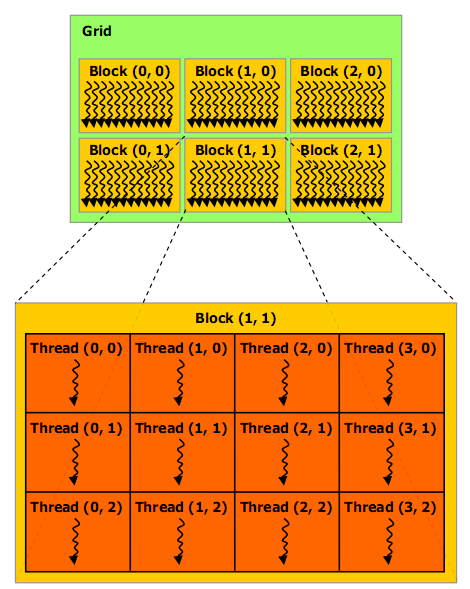
\includegraphics[width=.5\textwidth]{ThreadHierarchy.png}
	\caption{\label{fig:ThreadHierarchy} Jerarquía de hilos}
\end{figure}

\subsection{Jerarquía de Memoria}

Los hilos en CUDA pueden acceder a distintas memorias, unas compartidas y otras privadas. En primer lugar tenemos la memoria local privada de cada hilo. Cada bloque de hilos posee memoria compartida visible solo por los hilos del bloque y con el mismo tiempo de vida del bloque. Finalmente cada hilo en cada bloque de cada grid puede acceder a la memoria global.

\begin{figure}
	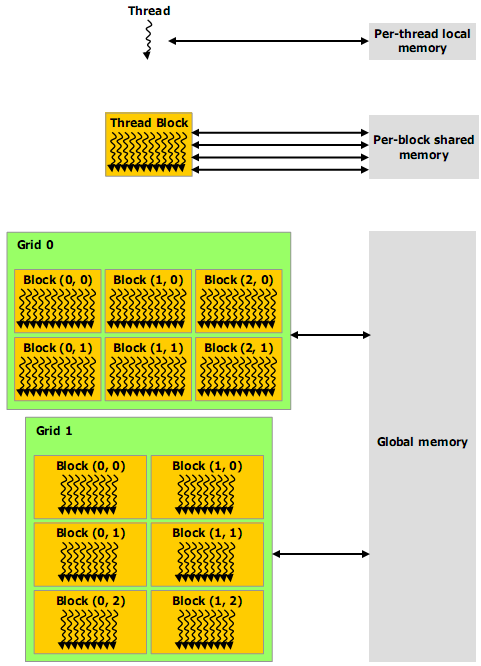
\includegraphics[width=.5\textwidth]{MemoriaHierarchy.png}
	\caption{\label{fig:MemoriaHierarchy} Jerarquía de memoria}
\end{figure}

Adicionalmente existen dos espacios de memoria de sólo lectura accesible por todos los hilos: la memoria de texturas y la memoria de constante, optimizadas para usos específicos. Las memorias global, de textura y constante persisten mientras el kernel permanezca en acción.

Asi como se puede identificar los hilos dentro de un bloque, se pueden identificar los bloques dentro de un grid, mediante una variable blockIdx que también puede ser un índice unidimensional, bidimensional o tridimensional.

\subsection{Sincronizaciones por Barrera}

Como los distintos hilos colaboran entre ellos y pueden compartir datos, se requieren directivas de sincronización. En CUDA se puede especificar una sincronización del tipo barrera, en la que todos los hilos esperan a que los demás lleguen al mismo punto.

\subsection{Kernel}

CUDA extiende el lenguaje permitiendo definir funciones llamadas kernels, que cuando son invocadas, son ejecutadas N veces en paralelo por N diferente hilos de CUDA.

Estas abstracciones permiten un granulado fino en el paralelismo de los datos y los hilos. Conduciendo al programador a dividir el problema en subproblemas que pueden ser tratados independientemente y en paralelo por bloques de hilos, y su vez dividir estos subproblemas en elementos individuales que pueden ser resueltos en paralelo y de manera cooperativa por todos los hilos de un mismo bloque.

Esta estructura preserva la expresividad del lenguaje permitiendo que los hilos cooperen en la resolución de cada subproblema, y al mismo tiempo permite la escalabilidad. En efecto, cada bloque de hilos puede ser programado en cualquier núcleo de procesamiento que este disponible, en cualquier orden, concurrente o secuencialmente. Por lo que cualquier programa CUDA ya compilado puede ejecutarse en sistemas con distinto numero de núcleos de procesamiento como se ilustra en la figura 3, y solo el sistema de tiempo de ejecución debe conocer el numero de núcleos físicos.

\begin{figure}
	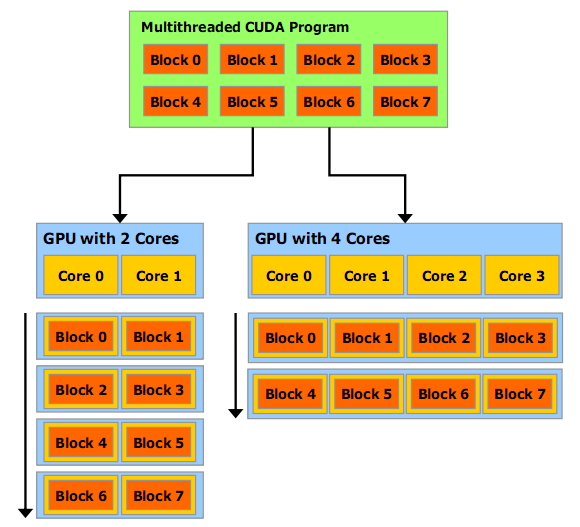
\includegraphics[width=.5\textwidth]{EscaladoGPU.png}
	\caption{\label{fig:EscaladoGPU} Escalado GPU}
\end{figure}

Todo esto desde el punto de vista del programador consiste en la extensión del lenguaje con un conjunto reducido de instrucciones, lo que supone un curva de aprendizaje suave.

\begin{center}
   \begin{tabular}{ | l | c | c | }
      \hline
      & \textbf{NVIDIA Tesla C2050} & \textbf{NVIDIA Tesla C1060} \\ \hline
      \textbf{Capacidad de cómputo} & 2.0 & 1.3 \\ \hline
      \textbf{Numero de Multiprocesadores/núcleos} & 14 (32 núcleos) & 30 (8 núcleos) \\ \hline
      \textbf{Total de Núcleos} & 448 & 240 \\ \hline
      \textbf{Memoria Global} & 2.62Gb & 4Gb \\ \hline
      \textbf{Memoria Compartida/bloque} & 48Kb & 16Kb \\ \hline
      \textbf{Máximo hilos/bloque} & 1024 & 512 \\ \hline
      \textbf{Dimensión Max. bloque} & 1024 x 1024 x 64 & 512 x 512 x 64 \\ \hline
      \textbf{Dimensión Max. grid} & 65535 x 65535 x 1 & 65535 x 65535 x 1 \\ \hline
      \textbf{Concurrencia de kernels} & disponible & no disponible \\
   \hline
   \end{tabular}
\end{center}

\section{Trabajo con PyCUDA}

\subsection{Primeras pruebas}

Durante el tiempo que hemos trabajado con PyCUDA en el último cuatrimestre, hemos implementado varios algoritmos de diferente complejidad. Inicialmente, nuestro objetivo consistió en familiarizarnos tanto con el entorno de trabajo como con una arquitectura que no habíamos empleado hasta ahora. Para ello, comenzamos escribiendo kernels que ejecutaban tareas sencillas tales como multiplicar un escalar por un vector, sumar dos vectores, etc. Este tipo de aplicaciones, aún cuando resultaron más eficientes ejecutados sobre la CPU que sobre la GPU en las mayoría de las pruebas --la gráfica solo alcanzaba mayor velocidad a partir de los 10.000 elementos-- , nos permitieron comprender la importancia de indicar el número adecuado de hilos por bloque o el tamaño del grid correcto tanto para acelerar el propio cálculo como para evitar los accesos no coalescentes a memoria. Huelga decir que en el caso anterior, la menor velocidad de la GPU se debe al tiempo empleado en la transferencia de datos de la memoria principal a la memoria del dispositivo y no al cómputo en sí.

\vspace{5 mm}

A continuación, abordamos dos problemas característicos: el producto matricial y la aplicación de un filtro de imagen. La manera tradicional de abordar la multiplicación de matrices pasa por ejecutar un algoritmo secuencial con un orden de complejidad casi cúbico en las mejores implementaciones. Dado que este algoritmo puede ser paralelizado sin mucha dificultad, nos planteamos su ejecución con PyCUDA para cruzar su eficiencia con la de su correspondiente versión de CPU. Nuestro banco de pruebas consistió en una serie de 8 multiplicaciones de matrices cuadradas generadas aleatoriamente. Las dimensiones de dichas matrices fueron incrementándose en 4 tras cada multiplicación, desde 4 hasta 32. Los datos obtenidos, que se recogen en el siguiente gráfico, muestran que la CPU solo fue más rápida en el caso de que las dos matrices tuvieran dimensión 4, mientras que el resto de los casos, no solo fue superior a la GPU (que se mantuvo prácticamente constante) sino que fue aumentando su distancia con ella a medida que el tamaño de las matrices se incrementaba.

\begin{center}
   \begin{figure}
      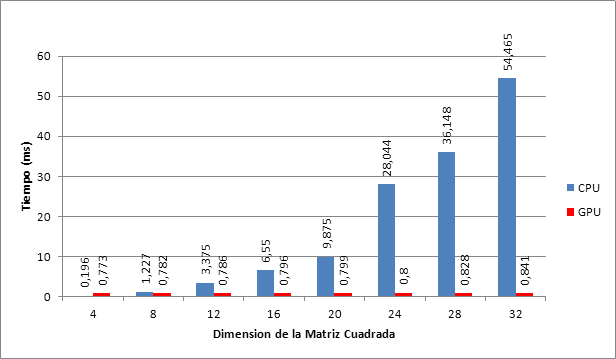
\includegraphics[width=.9\textwidth]{cpu-gpu.png}
      \caption{\label{fig:cpu-gpu}Eficiencia de cómputo: Producto matricial de NxN con algoritmo clásico O(n$^{3}$) frente a algoritmo paralelo sobre GPU}
   \end{figure}
\end{center}

En cuanto al filtro de imagen, nos decantamos por una implementación sencilla del filtro threshold consistente en examinar las componentes RGB de cada píxel de la imagen de entrada, saturándolo a blanco (255, 255, 255) si alguno de ellos presentaba un valor superior a 50. En este caso, comparamos la ejecución de este filtro consigo mismo, modificando sucesivamente los parámetros de la CUDA para, lanzando un hilo por cada píxel, comparar los resultados obtenidos con diferentes tamaños de bloque y de grid.

\subsection{Desarrollo del paquete \emph{Filters}}

Finalmente, escogimos como objetivo de desarrollo el diseño e implementación de un paquete que permita aplicar diferentes filtros a una imagen, a un conjunto de imágenes o a un vídeo, en cuyo caso será descompuesto en sus correspondientes frames. Este paquete puede utilizarse para acelerar el cálculo de aplicaciones complejas que requieran de la aplicación de filtros. En concreto, una de las más interesantes que hemos adaptado consiste en un programa de detección de movimiento.

\vspace{5 mm}

El paquete Filters se estructura, esencialmente, en torno a dos clases: CUDAHandler, concebido para comunicarse con la GPU, y Filter, clase abstracta de la que heredan cada uno de los filtros implementados. En la imagen adjunta, pueden observarse tres clases hijas de Filter que contienen las instrucciones para gestionar tres filtros necesarios para la detección de movimiento (Difference, Threshold y Erosion). Además, también se contempla una clase MotionDetection, encargada de realizar la detección en sí y que hace uso del paquete Filters, además de la clase VideoHandler que la abstrae de la manipulación de las operaciones de gestión de vídeo.

%%%%%%%%%%%%%%%%%%%%%%%%%%%

\begin{figure}
	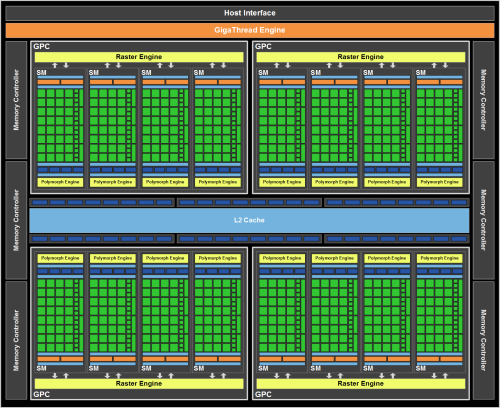
\includegraphics[width=.45\textwidth]{block_diagram_Fermi}
	\caption{\label{fig:Fermi} Diagrama de bloques de una GPU Tesla M2070 (Fermi)}
\end{figure}

y un código \ref{code:filter}

\lstinputlisting[%
   float=t,
   caption={Codigo de filtros en Python},
   label={code:filter} 
   ]%
   {code/filter.py}

\bibliographystyle{Jornadas}
\bibliography{memoria}

\end{document}

